
\hypertarget{working_database}{}
\section{Database}
\index{tools!database}

This interface
(Figure \ref{fig:tools_database_options})
contains resources related to the internal Tinn-R database.
Each tab (\textit{Shortcuts}, \textit{Completion} and
\textit{Comments}) has its own tool bar and pop-up menu allowing
for a fast control of the most common tasks.

\begin{figure}[h!]
  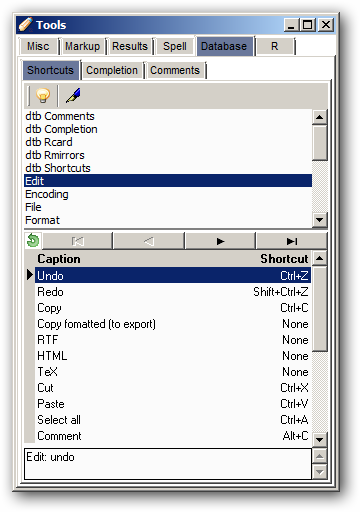
\includegraphics[scale=0.35]{./res/tools_database_shortcuts.png}~~
  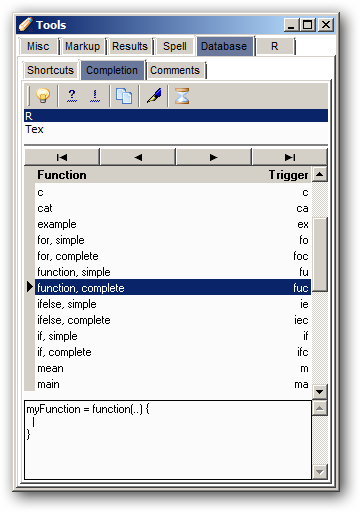
\includegraphics[scale=0.35]{./res/tools_database_completion.png}~~
  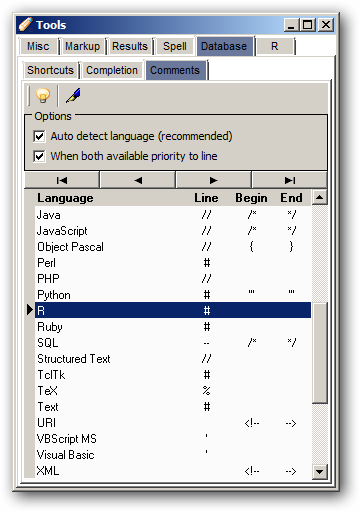
\includegraphics[scale=0.35]{./res/tools_database_comments.png}\\
  \caption{Database (Tools).}
  \label{fig:tools_database_options}
\end{figure}


\subsection{Shortcuts}
\index{tools!shortcuts}

\begin{figure}[h!]
  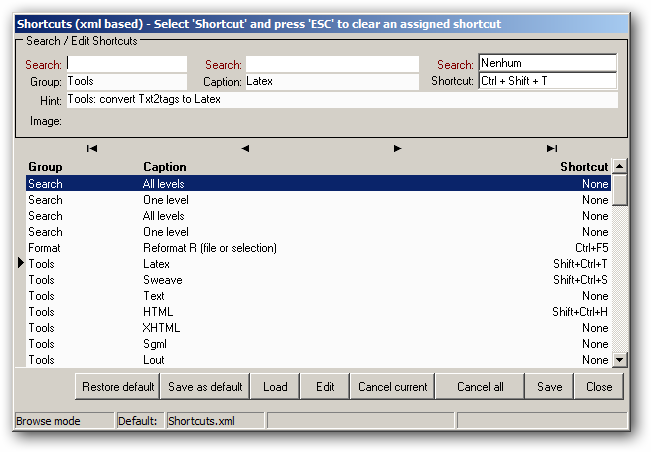
\includegraphics[scale=0.35]{./res/shortcuts_dlg.png}\\
  \caption{Shortcuts (Database).}
  \label{fig:shortcuts_dlg_2}
\end{figure}

The available buttons
(Figure \ref{fig:tools_database_options})
are:

\begin{quote}
  \begin{footnotesize}
    \begin{description}
      \item[Help:]
        It opens the \textit{User Guide} on the section about the selected topic.
      \item[Edit:]
        It opens the dialog \textit{R card database (xml based)} below.
    \end{description}
  \end{footnotesize}
\end{quote}

The \textit{Edit} button opens the dialog shown in Figure \ref{fig:shortcuts_dlg_2}.

Read below for a brief description of available buttons:

\begin{quote}
  \begin{footnotesize}
    \begin{description}
      \item[Restore default:]
        Restores the file \texttt{Shortcuts.xml} from the origin
        (InstallPath/data/data.zip). Any prior changes to the file
        \texttt{Shortcuts.xml} currently being used will be lost.
      \item[Save as default:]
        Opens the save dialog allowing you to save the file. From
        this point on, this file will be the new default shortcut.
      \item[Load:]
        Opens the open dialog allowing you to load a shortcut file.
        From this point on, this file will be the new default shortcut.
      \item[Edit:]
        Places the table in edition mode.
      \item[Cancel current:]
        Cancels any change made to the current edition.
      \item[Cancel all:]
        Cancels all changes made to the database prior to \textit{Save} or \textit{Save as default}.
      \item[Save:]
        Overwrites the text file (XML) saving all changes made to the current table.
      \item[Close:]
        Closes the dialog. All non-saved changes will be lost.
    \end{description}
  \end{footnotesize}
\end{quote}


\subsection{Completion}

\begin{figure}[h!]
  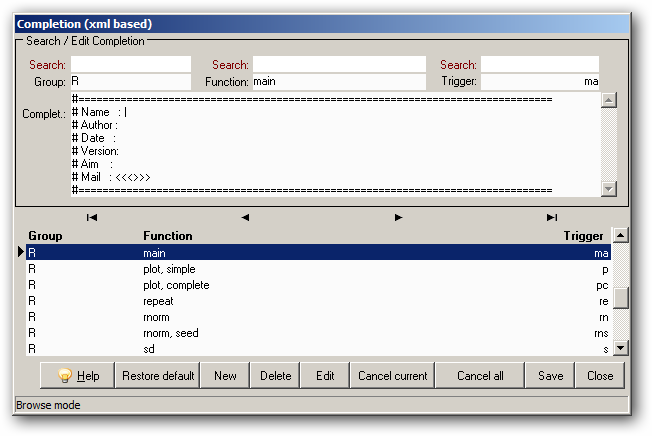
\includegraphics[scale=0.35]{./res/completion_dlg.png}\\
  \caption{Completion (Database).}
  \label{fig:completion_dlg}
\end{figure}

This resource adds a granular level of user customization for editing
functions within Tinn-R.

The completion (database based) allows the user to add functions based
on several programming languages such as \RR{}, \TeX, among others.

The available buttons
(Figure \ref{fig:tools_database_options})
are:

\begin{quote}
  \begin{footnotesize}
    \begin{description}
      \item[Help:]
        Sends the following instruction to \RR{}: \texttt{help('selected function')}.
      \item[Example:]
        Sends the following instruction to \RR{}:
        \texttt{example('selected function')}.
      \item[Copy function:]
        Places the selected function in the clipboard.
      \item[Copy description:]
        Places the description of the selected function in the clipboard.
      \item[Edit:]
        Opens the dialog \textit{Completion database (xml based)} below.
      \item[Insert:]
        Inserts the selected function in the active editor. A \texttt{Double click}
        or \texttt{Enter} performs the same function.
        The default shortcut is \texttt{CTRL + J}, but this can be customized under
        \textit{Options/Shortcuts} or \textit{Tools/Database/Shortcuts}. To use
        it just push the keystrokes after any valid word:

        \begin{verbatim}
          if<CTRL + J> to obtain:
          if (| < )

          ifc<CTRL + J> to obtain:
          if (| < ) {

          }

          fo<CTRL + J> to obtain:
          for (i in 1:i|)

          foc<CTRL + J> to obtain:
          for (i in 1:|) {

          }

          sw<CTRL + J> to obtain:
          switch(|,
          a = ' ',
          b = ' ',
          )

          wh<CTRL + J> to obtain:
          i = 0
          while (i < |) {

            i = i + 1
          }

          eq<CTRL + J> to obtain:
          \begin{equation}\label{eq_01}
            |
          \end{equation}
        \end{verbatim}

        \subsubsection{Observations:}
        \index{completion}
        \begin{enumerate}
          \item Only two letters were used to define the functions (for example:
            \textit{fo} = \textit{for}, \textit{fu} = \textit{function});
          \item Therefore, we added the letter \texttt{c} for more complex
            structures (for example: \textit{foc}, \textit{fuc});
          \item The \texttt{$|$} symbol is used to define where the cursor
            will first stop after auto-completion. After being selected
            the \texttt{$|$} symbol marks the point where the user can start
            typing.
        \end{enumerate}
    \end{description}
  \end{footnotesize}
\end{quote}

The \textit{Edit} button opens the dialog showed in the Figure \ref{fig:completion_dlg}.

Read below for a brief description of available buttons:

\begin{quote}
  \begin{footnotesize}
    \begin{description}
      \item[Restore default:]
        Restores the file \texttt{Completion.xml} from the origin at
        (\texttt{InstallPath/data/data.zip}). Any prior change to the file
        \texttt{Completion.xml} being used will be lost.
      \item[New:]
        Places the table in insertion mode.
      \item[Delete:]
        Deletes the current registry from the table.
      \item[Edit:]
        Places the table in edition mode.
      \item[Cancel current:]
        Cancels any change made to the current edition.
      \item[Cancel all:]
        Cancels all changes made to the database prior to \textit{Save}.
      \item[Save:]
        Overwrites the text file (XML), saving all changes made to the current table.
      \item[Close:]
        Closes the dialog. All non-saved changes will be lost.
    \end{description}
  \end{footnotesize}
\end{quote}


\subsection{Comments}

\begin{figure}[h!]
  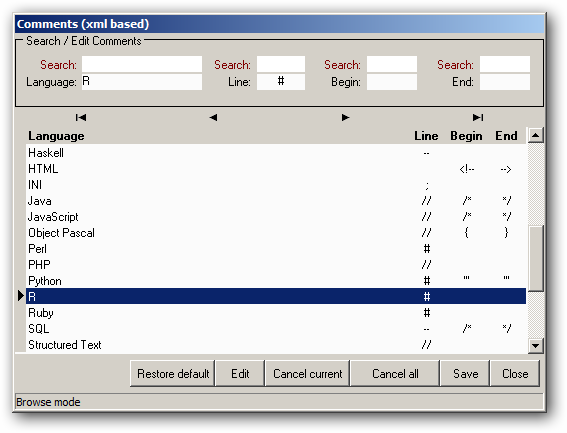
\includegraphics[scale=0.35]{./res/comments_dlg.png}\\
  \caption{Comments (Database).}
  \label{fig:comments_dlg}
\end{figure}

The available buttons
(Figure \ref{fig:tools_database_options})
are:

\begin{quote}
  \begin{footnotesize}
    \begin{description}
      \item[Help:]
        It opens the \textit{User Guide} on the section about the selected topic.
      \item[Edit:]
        It opens the dialog \textit{Comments (xml based)} below.
    \end{description}
  \end{footnotesize}
\end{quote}

The \textit{Edit} button opens the dialog shown in the Figure \ref{fig:comments_dlg}.

Read below a brief description of available buttons:

\begin{quote}
  \begin{footnotesize}
    \begin{description}
      \item[Restore default:]
        Restores the file \texttt{Comments.xml} from the origin at
        (\texttt{InstallPath/data/data.zip}). Any prior changes in the
        file \texttt{Comments.xml} currently being used will be lost.
      \item[Edit:]
        Places the table in edition mode.
      \item[Cancel current:]
        Cancels any change made to the current edition.
      \item[Cancel all:]
        Cancels all changes made to the database prior to \textit{Save}.
      \item[Save:]
        Overwrites the text file (XML) saving all changes made to the current table.
      \item[Close:]
        Closes the dialog. All non-saved changes will be lost.
    \end{description}
  \end{footnotesize}
\end{quote}
